\documentclass{zc-ust-hw}

\usepackage{lipsum}

\name{SalahDin Ahmed Salh Rezk}
\id{202201079}
\course{Introduction to Electronics (CIE 212)}
\assignment{Lab Assignment 3}

\begin{document}

\maketitle

\begin{enumerate}
  \item \,
    \begin{figure}[h]
      \centering
      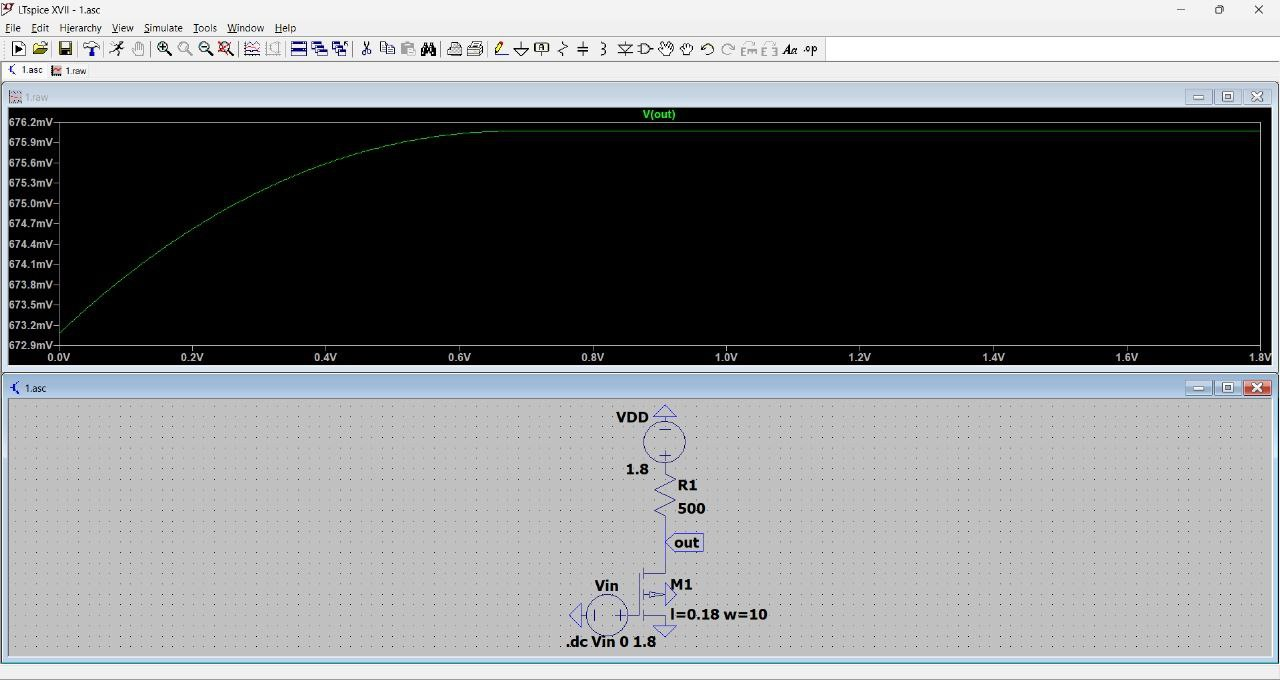
\includegraphics[width=\textwidth]{figures/1.jpg}
      \caption{}
    \end{figure}

    \begin{figure}[h]
      \centering
      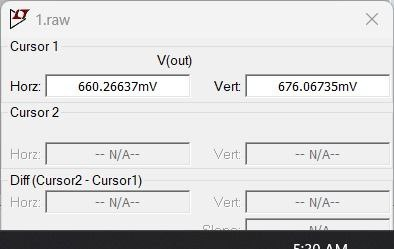
\includegraphics[width=0.5\textwidth]{figures/2.jpg}
      \caption{}
    \end{figure}

    The cursor shows that the value at which the slope reaches maximum is 0.66V.

    \newpage

  \item \,

    \begin{figure}[h]
      \centering
      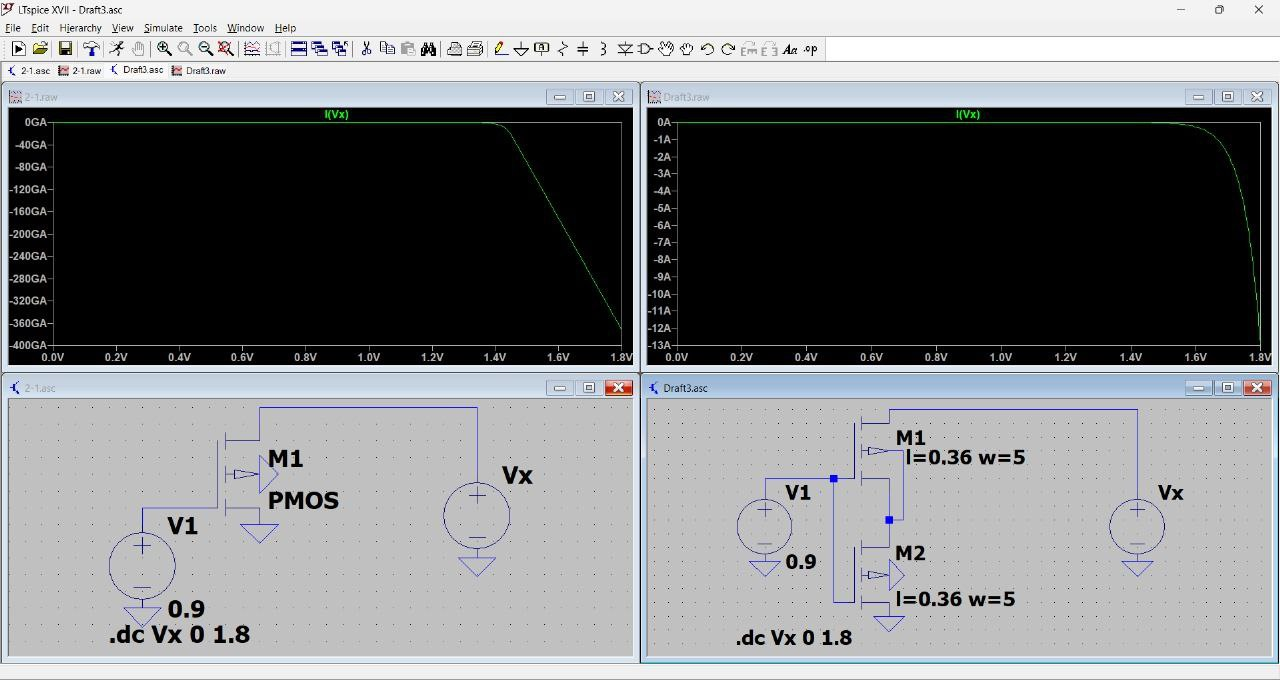
\includegraphics[width=\textwidth]{figures/cursor.jpg}
      \caption{}
    \end{figure}

    The two circuits are not equivalent the graph of the \( I_{x} \) is different for each one.


\end{enumerate}

\end{document}
